\documentclass[xcolor=x11names,compress]{beamer}

\usepackage{amssymb,graphicx}

\usetheme{Warsaw}
\usecolortheme{seahorse}

% Abbreviations
\newcommand{\bbC}{\mathbb{C}}
\newcommand{\bbD}{\mathbb{D}}
\newcommand{\bbH}{\mathbb{H}}
\newcommand{\bbN}{\mathbb{N}}
\newcommand{\bbR}{\mathbb{R}}
\newcommand{\bbZ}{\mathbb{Z}}
\newcommand{\calF}{\mathcal{F}}
\newcommand{\calS}{\mathcal{S}}
\newcommand{\gve}{\varepsilon}
\newcommand{\gvp}{\varphi}
\newcommand{\ga}{\alpha}
\newcommand{\gb}{\beta}
\newcommand{\gd}{\delta}
\newcommand{\gk}{\kappa}
\newcommand{\gl}{\lambda}
\newcommand{\glt}{\widetilde{\lambda}}
\newcommand{\go}{\omega}
\newcommand{\gr}{\gamma}
\newcommand{\grt}{\widetilde{\gamma}}
\newcommand{\gs}{\sigma}
\newcommand{\gt}{\theta}
\newcommand{\gz}{\zeta}
\newcommand{\gD}{\Delta}
\newcommand{\gR}{\Gamma}
\newcommand{\gL}{\Lambda}
\newcommand{\gO}{\Omega}
\renewcommand{\Re}{\text{Re}\,}
\renewcommand{\Im}{\text{Im}\,}
\newcommand{\area}{\text{area}}
\newcommand{\crad}{\text{crad}}
\newcommand{\diam}{\text{diam}}
\newcommand{\dist}{\text{dist}}
\newcommand{\length}{\text{length}}
\newcommand{\lcap}{\text{cap}}
\newcommand{\hcap}{\text{hcap}}
\newcommand{\rad}{\text{rad}}
\newcommand{\osc}{\text{osc}}
\newcommand{\half}{\frac{1}{2}}
\newcommand{\hypDist}{\rho_{\mathbb{D}}}
\newcommand{\Holder}{H\"{o}lder}
\newcommand{\supp}{\text{supp\,}}
\newcommand{\Lip}{\text{Lip}}
\newcommand{\Tip}{\text{Tip}}
\newcommand{\LipHalfNorm}{\mbox{$\Vert \gl \Vert_{\text{Lip}(\frac{1}{2})}$}}
\newcommand{\LipHalfNormt}{\mbox{$\Vert \widetilde{\gl} \Vert_{\text{Lip}(\frac{1}{2})}$}}
\newcommand{\MTdeltaCondition}{$(M,T,\delta)$-Lip($\frac{1}{2}+\delta$) condition}
\newcommand{\sigmaCondition}{$\sigma$-Lip($\frac{1}{2}$) condition}
\newcommand{\MTnAlphaCondition}{$(M,T,n,\alpha)$-$C^{n,\alpha}$ condition}
\newcommand{\MToneDeltaCondition}{$(M,T,1,\delta)$-$C^{1,\delta}$ condition}

% Environments
\theoremstyle{definition}
\newtheorem*{conjecture}{Conjecture}
\newtheorem*{question}{Question}
\newtheorem*{answer}{Answer}
\newtheorem*{exercise}{Exercise}
\newtheorem*{remark}{Remark}

\title{Smoothness of Loewner Slits}
\author{Carto Wong}
\institute{University of Washington}
\date{Nov 9, 2010}

\begin{document}

\maketitle

\section{Background}

\begin{frame}
  \frametitle{Chordal Loewner differential equation}
  Let $\bbH = \{ \Im z > 0 \}$ be the upper halfplane.
  \begin{itemize}
    \item  A slit in $\bbH$ is a simple curve $\gr \colon (0,T] \to \bbH$ with base $\gr(0) \in \bbR$.
    \item  $g_t \colon H_t \to \bbH$ is a conformal mapping from $H_t = \bbH \setminus \gr([0,t])$ onto $\bbH$.
  \end{itemize}
  \vspace{.1in}
  Hydrodynamic normalization:
  \[
      g_t(z) = z + \frac{2t}{z} + \cdots \qquad (z \to \infty)
  \]
  \begin{figure}
    \includegraphics[scale=0.8]{figures/pdf/g(t,z).pdf}
  \end{figure}
\end{frame}

\begin{frame}
  \frametitle{Chordal Loewner differential equation}
  \begin{theorem} \label{Thm:chordalLoewnerEqt}
    $g_t(z)$ satisfies
    \[
      \partial_t g_t(z) = \frac{2}{g_t(z) - \gl(t)},
    \]
    for all $z \in H_t = \bbH \setminus \gr([0,t])$, where $\gl \colon [0,T] \to \bbR$ is a continuous function. Moreover,
    $\gl(t) = g_t(\gr(t))$.
  \end{theorem}
  \begin{figure}
    \includegraphics[scale=0.8]{figures/pdf/chordalLE.pdf}
  \end{figure}
\end{frame}

\begin{frame}
  \begin{example}
    vertical slit $\gr(t) = 2i \sqrt{t}$
    \[
        \begin{aligned}
           g_t(z) &= \sqrt{z^2 + 4t} \\
           \partial_t g_t(z) &= \frac{2}{\sqrt{z^2 + 4t}} = \frac{2}{g_t(z)}
       \end{aligned}
    \]
    So, $\gl(t) \equiv 0$ for the vertical slit.      
  \end{example}
  \begin{figure}
    \includegraphics[scale=0.8]{figures/pdf/verticalSlit.pdf}
  \end{figure}
\end{frame}

\begin{frame}
  We have a map
  \[
    \left\{ \begin{aligned} 
      &\text{slits in the upper}\\
      &\text{halfplane } \bbH\ \text{modulo}\\
      &\text{reparametrization}
    \end{aligned} \right\}  
    \longrightarrow
    \left\{ \begin{aligned}
      &\text{continuous functions}\\
      &\gl \colon [0,T] \to \bbR
    \end{aligned} \right\}
  \]  
  which is 1-1, but not onto.

  \begin{figure}
    \includegraphics[scale=0.6]{figures/pdf/LE_relation.pdf}
  \end{figure}
  
  Kufarev gave an example (in the disc case) of a continuous $\gl(t)$ which does not generate slit. 
\end{frame}

\begin{frame}
  \begin{question}
    When does $\gl \colon [0,T] \to \bbR$ generate slit?
  \end{question}
  
  \begin{itemize}
    \item  (Kufarev) If $\gl$ is $C^1$, then it generates a slit.
    \item  (Marshall, Rohde 2005) If $\LipHalfNorm < c_0$, then it generates a quasi-slit in $\bbH$.
    \item  (Lind 2005) The best constant is $c_0 = 4$.  
  \end{itemize}
  
  \begin{question}
    What more can we say if $\gl$ is more regular than $\Lip(\half)$?
  \end{question}
  \begin{itemize}
    \item (see [Ale]) If $\gl$ has bounded first derivative, then $\gr$ is $C^1$. 
  \end{itemize}
  [Ale]  I. A. Aleksandrov, Parametric continuations in the theory of univalent functions, Izdat. �Nauka, 1976.  
\end{frame}

\begin{frame}
  \frametitle{1st main result}
  \begin{theorem}[W- 2010] 
    Suppose $\gl \colon [0,T] \to \bbR$ is $\Lip(\half + \gd)$ with $0 < \gd \leq \half$. Then
    \begin{enumerate}
      \renewcommand{\theenumi}{\alph{enumi}}
      \item  $\gr(t^2)$ is $C^{1,\gd}$ regular on $[0,T]$.
      \item  $\gr(t)$ grows vertically at $t = 0$ and
                 \[
                     \left| \gr'(t) - \frac{i}{\sqrt{t}} \right| \leq N t^{-\half + \gd}
                 \]
                 where $N > 0$ is a constant.
    \end{enumerate}
    With an extra assumption $\LipHalfNorm \leq 1$, both statements are quantitative.
  \end{theorem}
\end{frame}

\begin{frame}
  \frametitle{2nd main result}
  \begin{theorem}[W- 2010]
    Let $\gl \colon [0,T] \to \bbR$ and $0 < \gd \leq \half$.
    \begin{enumerate}
      \renewcommand{\theenumi}{\alph{enumi}}
      \item  If $\gl$ is $C^{1,\gd}$, then $\gr$ is $C^{1,\half + \gd}$ regular on $(0,T]$.
      \item  If $\gl$ is $C^{1,\half+\gd}$, then $\gr$ is $C^{2, \gd}$ regular on $(0,T]$.
    \end{enumerate}
    With an extra assumption $\LipHalfNorm \leq 1$, both statements are quantitative.
  \end{theorem}
  \vspace{.2in}  
  Roughly speaking, $\gl \in C^{n+\ga} \Rightarrow \gr \in C^{n+\half+\ga}$ for $n + \ga \leq 2$.
\end{frame}

\begin{frame}
  \frametitle{LE diagram}
  \begin{figure}
    \includegraphics[scale=0.8]{figures/pdf/LE_relation.pdf}
  \end{figure}
  If we modify one picture,
  \begin{itemize}
    \item  how does the other change?
    \item  {\color{gray!30} how do we quantify and estimate the change?}
  \end{itemize}
\end{frame}

\begin{frame}
  \frametitle{LE diagram}
  \begin{figure}
    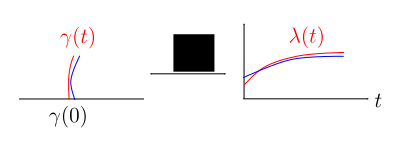
\includegraphics[scale=0.8]{figures/pdf/mod_cont.pdf}
  \end{figure}
  If we modify one picture,
  \begin{itemize}
    \item  how does the other change?
    \item  how do we quantify and estimate the change?
  \end{itemize}
\end{frame}

\begin{frame}
  \frametitle{Stationary property}
  \begin{figure}
    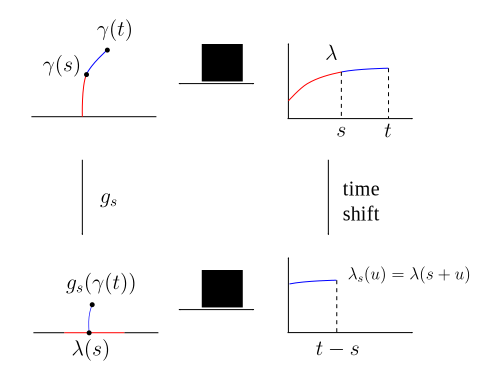
\includegraphics[scale=0.5]{figures/pdf/stationary.pdf}
  \end{figure}
  \begin{proof}
    $\partial_u g_{s+u}(z) = \frac{2}{g_{s+u}(z) - \gl(s+u)}$. 
  \end{proof}
\end{frame}

\begin{frame}
  \frametitle{Scaling property}
  \begin{figure}
    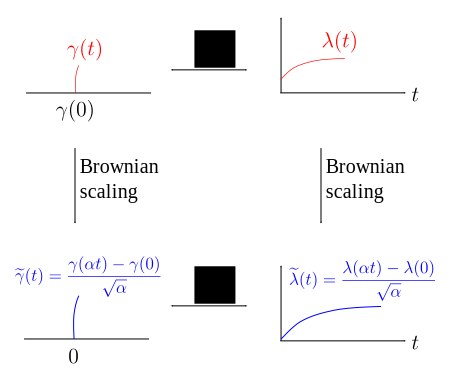
\includegraphics[scale=0.5]{figures/pdf/scaling.pdf}
  \end{figure}
  \begin{proof}
    $\partial_t \left[ \frac{1}{\sqrt{\ga}} g_{\ga t}(\sqrt{\ga} z) \right] =
    \frac{2}{\frac{1}{\sqrt{\ga}} g_{\ga t}(\sqrt{\ga} z) - \frac{1}{\sqrt{\ga}} \gl(\ga t)}$.  
  \end{proof}
\end{frame}

\section{$\gl \in \Lip(\half)$}

\begin{frame}
 For $0 \leq \gs < 4$, let
 \[
     X_{\gs} = \left\{ \gl \colon [0,1] \to \bbR \text{ with } \gl(0) = 0 \text{ and } \LipHalfNorm \leq \gs \right\}
 \]
 $(X_{\gs}, \Vert \cdot \Vert_{\infty})$ is a compact metric space and
 \[
     \begin{aligned}
       \Tip \colon X_{\gs} &\to \bbH \\
       \gl &\mapsto \gr(1)
     \end{aligned}  
 \]
 is continuous, and therefore has a compact image $E_{\gs} = \Tip(X_{\gs})$.
  \begin{figure}
    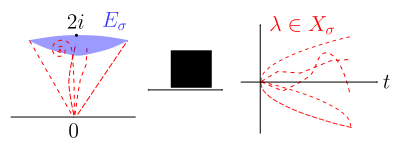
\includegraphics{figures/pdf/diamE.pdf}
  \end{figure}
\end{frame}

\begin{frame}
  \frametitle{Two lemmas concerning $\Tip \colon X_{\gs} \to \bbH$}
  \begin{lemma}[size of the image]
    $\diam \, E_{\gs} = O(\gs)$ as $\gs \to 0$.
  \end{lemma}

  \begin{figure}
    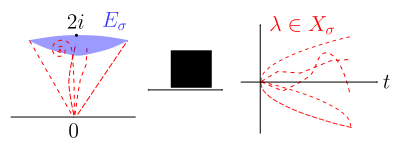
\includegraphics[scale=0.6]{figures/pdf/diamE.pdf}
  \end{figure}
  
  \begin{lemma}[modulus of continuity]
    If $\Vert \gl_j \Vert_{\Lip(\half)} \leq 1$, then
    \[
        \left| \Tip(\gl_1) - \Tip(\gl_2) \right| \leq c \Vert \gl_1 - \gl_2 \Vert_{\infty}.
    \]
  \end{lemma}
\end{frame}

\section{$\gl \in \Lip(\half + \gd)$}

\begin{frame}
  \frametitle{Slit grows vertically}
  \[
    \begin{aligned}
      \gl \in \Lip(\half) &\Rightarrow \gr(t) \in \sqrt{t} E_{\gs} \\
     \gl \in \Lip(\half + \gd) &\Rightarrow \gr(t) \in \sqrt{t} E_{\gs(t)} \text{ with } \gs(t) = O(t^{\gd})
   \end{aligned}
 \]    
  \begin{figure}
    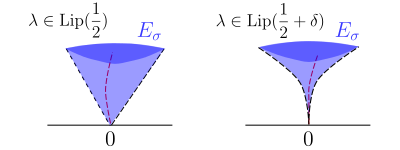
\includegraphics[scale=0.8]{figures/pdf/vertically.pdf}
  \end{figure}
\end{frame}

\begin{frame}
  \frametitle{1st main result}
  \begin{theorem}[W- 2010] 
    Suppose $\gl \colon [0,T] \to \bbR$ is $\Lip(\half + \gd)$ with $0 < \gd \leq \half$. Then
    \begin{enumerate}
      \renewcommand{\theenumi}{\alph{enumi}}
      \item  {\color{gray!30} $\gr$ is $C^{1,\gd}$ regular on $(0,T]$.}
      \item  $\gr(t)$ grows vertically at $t = 0$ \checkmark {\color{gray!30} and
                 \[
                     \left| \gr'(t) - \frac{i}{\sqrt{t}} \right| \leq N t^{-\half + \gd}
                 \]
                 where $N > 0$ is a constant.}
    \end{enumerate}
    {\color{gray!30} With an extra assumption $\LipHalfNorm \leq 1$, both statements are quantitative.}
  \end{theorem}
\end{frame}

\begin{frame}
  \frametitle{Existence of $\gr'(s)$}
  Suppose $\gl_j \colon [0,T] \to \bbR$ ($j$ = 1, 2) satisfy
  \[
      \left\{ \begin{aligned}
        &\left| \gl_j(t_1) - \gl_j(t_2) \right| \leq M \left| t_1 - t_2 \right|^{\half + \gd} \\
        &\gl_1 = \gl_2 \text{ on } [0,s]
      \end{aligned} \right.  
  \]
  Then $\left| \gr_1(s+\gve) - \gr_2(s+\gve) \right| = O(\gve^{?})$ as $\gve \to 0+$.
  \begin{figure}
    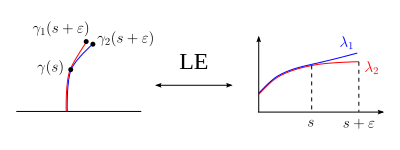
\includegraphics[scale=1]{figures/pdf/slitApprox.pdf}
  \end{figure}
\end{frame}

\begin{frame}
  \frametitle{Existence of $\gr'(s)$}
  Fix $\gl_1 \colon [0,s] \to \bbR$ and let
  \[
      K_{\gve} = \left\{ \gr^{\gl}(s+\gve) \in \bbH \; \middle\vert
      \begin{aligned}
        &\gl \colon [0,s+\gve] \to \bbR \text{ satisfying } \gl = \gl_1 \text{ on } [0,s] \\
        &\text{and } \sup_{t_1 \not= t_2 \in [0,T]} \frac{\left| \gl(t_1) - \gl(t_2) \right|}{\left| t_1 - t_2 \right|^{\half + \gd}} \leq M
      \end{aligned} \right\}   
  \]
  \begin{figure}
    \includegraphics[scale=0.5]{figures/pdf/slitApproxSol.pdf}
  \end{figure}
\end{frame}

\begin{frame}
  \frametitle{Existence of $\gr'(s)$}
  \begin{lemma} \label{L:f'_Lip(1/2+delta)}
    Suppose $\gl \colon [0,T] \to \bbR$ satisfies
    \begin{itemize}
      \item  the \MTdeltaCondition\ for some $0 < \gd \leq \half$; and
      \item $\LipHalfNorm \leq 1$
    \end{itemize}  
    {\color{gray!50} then for any $0 < s < t \leq T$,
    \[
        \frac{1}{C} \leq \sqrt{\frac{t-s}{t}} \left| g_s'(\gr(t)) \right| \leq C,
    \]
    where $C = C(M, T, \gd) > 0$.} Moreover, for all $s \in (0,T)$, the limit
    \[
        \lim_{\gve \to 0+} \sqrt{\gve} g_s'(\gr(s+\gve)) = {\color{gray!50} \sqrt{s}
        \exp \left[ - \int_0^s \frac{1}{2u} + \frac{2}{\gr(s-u,s)^2} \, du \right]}
    \]
    exists and is nonzero.
  \end{lemma}
\end{frame}

\begin{frame}
  \frametitle{Existence of $\gr'(s)$}
  For $\gl \in Lip(\half + \gd)$, the lemma says $\left| g_s'(\gr(s+\gve)) \right| \asymp \gve^{- \half}$. Near the tip
  $\gr(s)$ the slit halfplane cannot have a ``corner of angle strictly less than $2\pi$''.
  \begin{figure}
    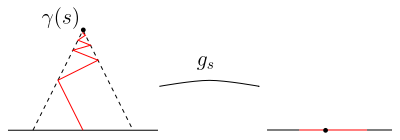
\includegraphics{figures/pdf/corner.pdf}
  \end{figure}
\end{frame}

\begin{frame}
  \frametitle{Existence of $\gr'(s)$}
   \[
      \diam \, K_{\gve} \lesssim \diam[ g_s(K_{\gve})] \cdot \sup_{z} \left| g_s^{-1}(z) \right| \lesssim
      \gve^{1 + \gd}.  
  \]
  \begin{figure}
    \includegraphics[scale=0.5]{figures/pdf/slitApproxSol.pdf}
  \end{figure}
\end{frame}

\begin{frame}
  \frametitle{Existence of $\gr'(s)$}
  Given $\gl \in \Lip(\half + \gd)$, modify $\gl$ so that it is constant after time $s$. This does not change the existence
  and the value of
  \[
      \lim_{\gve \to 0+} \frac{\gr(s+\gve) - \gr(s)}{\gve}.
  \]
  Can assume $\gr(s+\gve) = f_s( \gl(s) + 2i\sqrt{\gve})$, where $f_s = g_s^{-1}$.
  \begin{figure}
    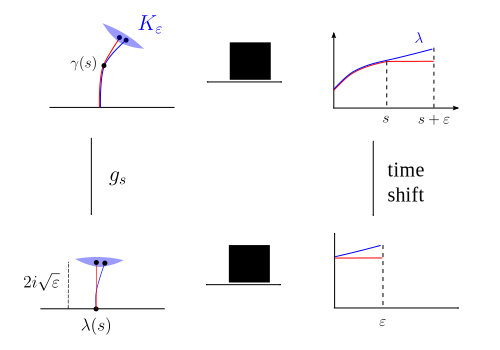
\includegraphics[scale=0.5]{figures/pdf/constantApprox.pdf}
  \end{figure}
\end{frame}

\begin{frame}
  \frametitle{Existence of $\gr'(s)$}
  \begin{corollary}
    Assuming the \MTdeltaCondition\ and $\LipHalfNorm \leq 1$, for any $0 < s \leq T$ we have
    \[
        \gr'(s) = \frac{i}{\sqrt{s}} \exp \left[ \int_0^s \frac{1}{2u} + \frac{2}{\gr(s-u,s)^2} \, du \right],
    \]
    where $\gr(s-u,s) = g_{s-u}(\gr(s)) - \gl(s-u)$.
  \end{corollary}
  
  \begin{figure}
    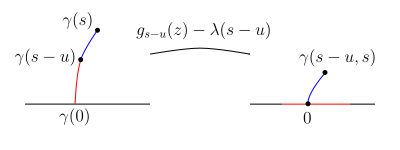
\includegraphics[scale=0.8]{figures/pdf/r(s-u,s).pdf}
  \end{figure}
\end{frame}  

\begin{frame}  
  $\gr'(s) = \frac{i}{\sqrt{s}} e^{L(s)}$ is equally regular as the function
  \[
      L(s) = \int_0^s \frac{1}{2u} + \frac{2}{\gr(s-u,s)^2} \, du.
  \]
  For $\gl \in \Lip(\half + \gd)$, we can show $L \in \Lip(\gd)$ by estimating
  \[
      \begin{aligned}
        L(s+\gve) - L(s)  
        = &\int_0^s \frac{2}{\gr(s+\gve-u,s+\gve)^2} - \frac{2}{\gr(s-u,s)^2} \, du +\\
        &\int_s^{s+\gve}  \frac{1}{2u} + \frac{2}{\gr(s+\gve-u,s+\gve)^2}  \, du. \\
      \end{aligned}
  \]
\end{frame}

\section{more...}

\begin{frame}
  \frametitle{Current progress}
  All driving functions below are assumed to satisfy $\LipHalfNorm \leq 1$. Let
  $0 < \delta \leq \half$.
  \begin{itemize}
    \item  If $\gl \in C^{1,\gd}$, then $L$ is $\Lip(\half+\gd)$
               and therefore $\gr$ is $C^{1,\half+\gd}$.
    \item  If $\gl \in C^{1,\half+\gd}$, then
               \[
                  \gr''(s) = \frac{2 \gr'(s)}{\gr(s)^2} - 4 \gr'(s) Q(s)
               \]
               where $Q \in \Lip(\gd)$ and is given by
               \[
                  Q(s) := \int_0^s \frac{\partial_s \gr(s-u,s)}{\gr(s-u,s)^3}  \, du.
               \]
               It means that $\gr$  is $C^{2,\gd}$.
  \end{itemize}
\end{frame}

\begin{frame}
  \frametitle{Unsolved problem}
  \begin{itemize}
    \item Conjecture: If $\gl \in C^{n+\ga}$ then $\gr \in C^{n+\half+\ga}$.
              \vspace{.1in} \newline
              Proved for $n+\ga \leq 2$. \vspace{.2in}
    \item The converse statement: if $\gr \in C^{n,\ga}$, how smooth is $\gl$?
              \vspace{.1in} \newline
              C. Earle, A. Epstein: if $\gr \in C^n$ ($n \geq 2$), then $\gl \in C^{n-1}$.              
  \end{itemize}
\end{frame}

\begin{frame}
  \begin{center}
    \huge{Thank you!}
  \end{center}  
\end{frame}

\end{document}
